\documentclass{article}

% Required package for including images (handles .png, .jpg, .pdf, etc.)
\usepackage{graphicx}

\usepackage{geometry}
\geometry{a4paper, margin=1in}
\usepackage{caption}

\title{Analysis of a Coin-Flip Game Simulation}
\author{Tashfeen Omran}
\date{\today}

\begin{document}

\maketitle

\section{Introduction}

This document analyzes the results of a Monte Carlo simulation of a simple coin-flipping game. The simulation visualizes the potential outcomes and profit distributions of the game. The generated plot is included and centered in the following section.

\section{Simulation Results}

The figure below illustrates the outcomes of the simulation. The top plot shows the cumulative profit over a series of flips, while the bottom plot shows a histogram of the final profits from all simulations.

% The 'figure' environment with the \centering command
% is the standard way to insert and center an image.
\begin{figure}[!htbp]
    \centering
    
    % Include the PNG file directly.
    % Ensure 'coin_flip_simulation.png' is in the same folder as your .tex file.
    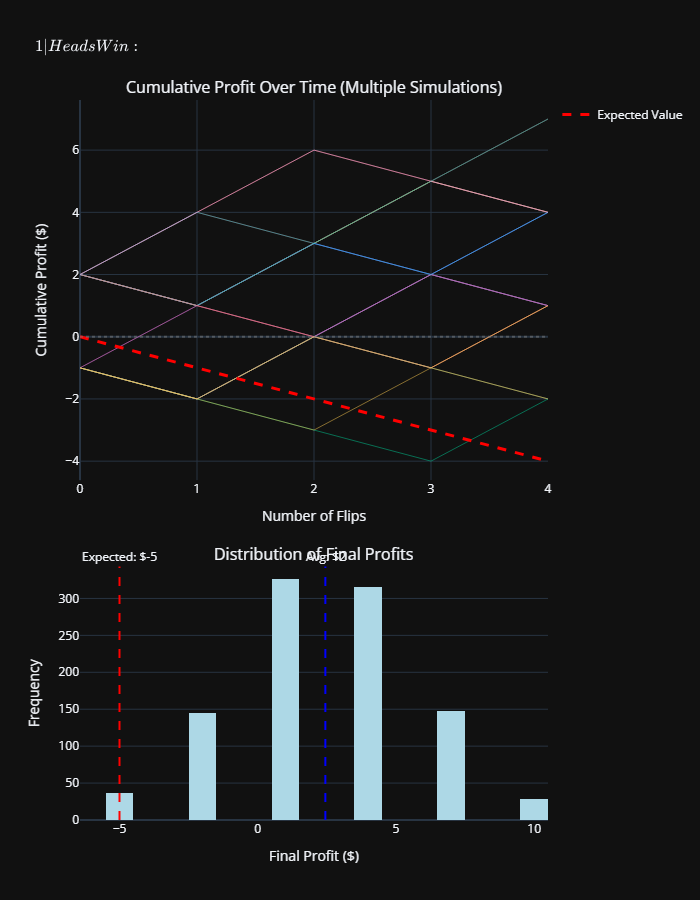
\includegraphics[width=\textwidth]{coin_flip_simulation.png}
    
    \caption{A Monte Carlo simulation of a coin-flip game, displaying both the cumulative profit paths and the final profit distribution.}
    \label{fig:coin_simulation}
\end{figure}

\section{Conclusion}

As demonstrated in Figure~\ref{fig:coin_simulation}, the simulation provides valuable insights into the risk and reward of the game. This visualization is key to understanding the range of possible outcomes.

\end{document}